\documentclass[tikz,border=5pt]{standalone}
\usepackage{ctex,amsmath}
\usetikzlibrary{arrows.meta,calc}
\tikzset{>=Latex,hose/.style={blue!65!black,thick},guide/.style={gray!65,thin},force/.style={orange!85!black,very thick,->},motion/.style={green!40!black,thick,->}}
% 单条连续螺线，外缘终点位于下方，端点径向导数为零，切向连接地面段。
\newcommand{\coil}[3]{
\begin{scope}[shift={(#1,#2)}]
\fill[blue!3](0,0)circle(#3);
\draw[guide,dashed](0,0)circle(#3);
\draw[hose]plot[domain=0:1,variable=\t,samples=1001]
({#3*(.08+.92*(\t-sin(360*\t)/(2*pi)))*cos(2520*\t-90)},
 {#3*(.08+.92*(\t-sin(360*\t)/(2*pi)))*sin(2520*\t-90)});
\end{scope}}
\begin{document}
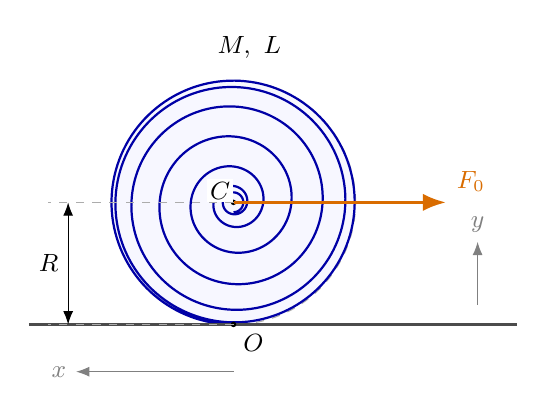
\begin{tikzpicture}[font=\small]
\coil{0}{1.55}{1.55}
\draw[black!70,thick](-2.6,0)--(3.6,0);
\fill(0,1.55)circle(.035)node[above left,fill=white,inner sep=1pt]{$C$};
\fill(0,0)circle(.035)node[below right]{$O$};
\draw[force](0,1.55)--(2.7,1.55)node[above right]{$F_0$};
\draw[guide,dashed](0,1.55)--(-2.35,1.55);
\draw[guide,dashed](0,0)--(-2.35,0);
\draw[<->](-2.10,0)--(-2.10,1.55)node[midway,left]{$R$};
\node[above]at(.2,3.25){$M,\ L$};
\draw[gray,->](0,-.6)--(-2,-.6)node[left]{$x$};
\draw[gray,->](3.1,.25)--(3.1,1.05)node[above]{$y$};
\end{tikzpicture}
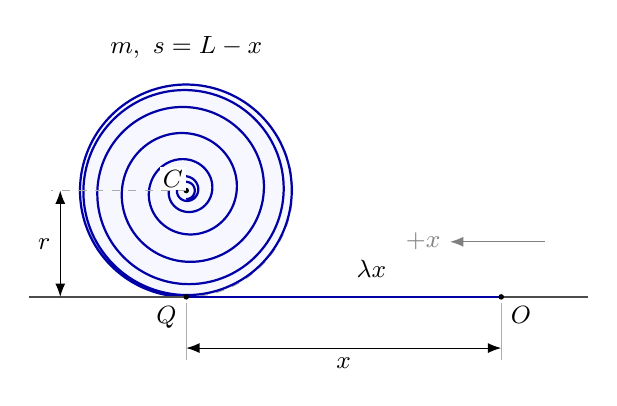
\begin{tikzpicture}[font=\small]
\coil{-4}{1.35}{1.35}
\draw[black!70,thick](-6,0)--(1.1,0);
\draw[hose](-4,0)--(0,0);
\fill(-4,1.35)circle(.035)node[above left,fill=white,inner sep=1pt]{$C$};
\fill(-4,0)circle(.035)node[below left]{$Q$};
\fill(0,0)circle(.035)node[below right]{$O$};
\draw[guide,dashed](-4,1.35)--(-5.72,1.35);
\draw[<->](-5.6,0)--(-5.6,1.35)node[midway,left]{$r$};
\draw[<->](-4,-.65)--(0,-.65)node[midway,below]{$x$};
\draw[guide](-4,-.08)--(-4,-.8)(0,-.08)--(0,-.8);
\node[above]at(-4,2.9){$m,\ s=L-x$};
\node[above]at(-1.65,.12){$\lambda x$};
\draw[gray,->](.55,.7)--(-.65,.7)node[left]{$+x$};
\end{tikzpicture}
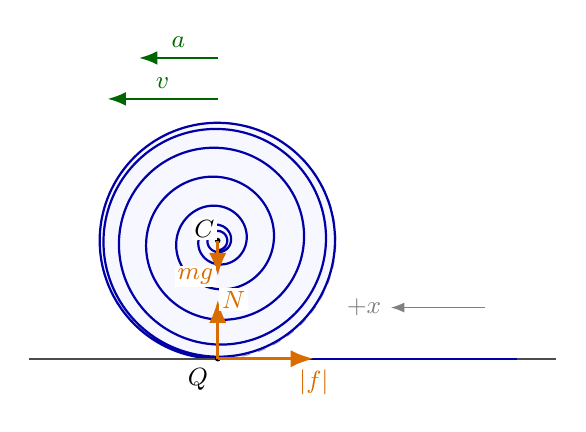
\begin{tikzpicture}[font=\small]
\coil{-2}{1.5}{1.5}
\draw[black!70,thick](-4.4,0)--(2.3,0);
\draw[hose](-2,0)--(1.8,0);
\fill(-2,1.5)circle(.035)node[above left,fill=white,inner sep=1pt]{$C$};
\fill(-2,0)circle(.035)node[below left]{$Q$};
\draw[force](-2,0)--(-2,.75)node[right,fill=white,inner sep=1pt]{$N$};
\draw[force](-2,1.5)--(-2,1.05)node[left,fill=white,inner sep=1pt]{$mg$};
\draw[force](-2,0)--(-.78,0)node[below]{$|f|$};
\draw[motion](-2,3.30)--(-3.4,3.30)node[midway,above]{$v$};
\draw[motion](-2,3.82)--(-3.0,3.82)node[midway,above]{$a$};
\draw[gray,->](1.4,.65)--(.2,.65)node[left]{$+x$};
\end{tikzpicture}
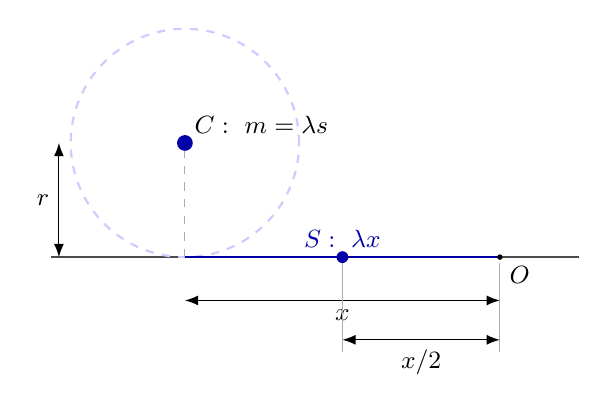
\begin{tikzpicture}[font=\small]
\draw[black!70,thick](-5.7,0)--(1,0);
\draw[blue!20,thick,dashed](-4,1.45)circle(1.45);
\draw[hose](-4,0)--(0,0);
\draw[guide,dashed](-4,0)--(-4,1.45);
\fill[blue!65!black](-4,1.45)circle(.10);
\node[above right]at(-4,1.45){$C:\ m=\lambda s$};
\fill[blue!65!black](-2,0)circle(.075)node[above]{$S:\ \lambda x$};
\fill(0,0)circle(.035)node[below right]{$O$};
\draw[<->](-4,-.55)--(0,-.55)node[midway,below]{$x$};
\draw[<->](-2,-1.05)--(0,-1.05)node[midway,below]{$x/2$};
\draw[guide](0,-.08)--(0,-1.2)(-2,-.08)--(-2,-1.2);
\draw[<->](-5.6,0)--(-5.6,1.45)node[midway,left]{$r$};
\end{tikzpicture}
\begin{tikzpicture}[font=\small]
\draw[black!70,thick](-5.6,0)--(1.1,0);
\draw[blue!20,thick,dashed](-4,1.45)circle(1.45);
\draw[hose](-4,0)--(0,0);
\fill(-4,1.45)circle(.04)node[above right]{$C$};
\fill(0,0)circle(.04)node[below right]{$O$};
\draw[guide,dashed](-4,1.45)--(0,1.45)--(0,0);
\draw[force](-4,1.45)--(-5.3,1.45)node[left]{$P_x$};
\draw[force](-4,1.45)--(-4,.45)node[right]{$|P_y|$};
\draw[<->](-4,-.6)--(0,-.6)node[midway,below]{$x$};
\draw[<->](.4,0)--(.4,1.45)node[midway,right]{$r$};
\draw[green!40!black,thick,->](-3.22,2.20)arc[start angle=45,end angle=160,radius=1.1];
\node[green!40!black,above]at(-4,2.74){$L_C>0$};
\node[below]at(-2,-1.05){逆时针为正};
\end{tikzpicture}
\end{document}
